\chapter{Symmetries, Tight-Binding Band Structure Theory, and Effective Models}

Last time we built second quantization and put it to work: mean-field theory turned an
interacting, quartic Hamiltonian into an effective single-particle one, and we watched that same
recipe produce a charge density wave, a magnet, and a superconductor, one for each of the three
symmetries a many-body ground state can spontaneously break. We spent real time on what that
breaking actually means: the bread-on-the-table picture of a set of equally good solutions with no
individual realization respecting the full symmetry, the requirement that this only becomes sharp
in the thermodynamic limit, the ferroelectric as a fourth worked example alongside magnets and
superconductors, and the contrast with topological order, which can tell two materials apart with
identical broken symmetries. That is a complete story in itself, and today's session is not going
to repeat any of it.

Instead, today asks a different, more structural question. Once interactions have been packaged
away into a mean-field, single-particle Hamiltonian, how do we actually solve it? For a handful of
sites we can diagonalize a matrix by brute force, but a real material has of order $10^{23}$ sites,
and no computer will ever diagonalize that directly. The answer, once again, is symmetry, but used
in a different role than last time: not to classify which order a ground state breaks, but to
simplify the diagonalization itself. When the ground state of a Hamiltonian actually \emph{shares} the
Hamiltonian's symmetry, that symmetry stops being a classification tool and becomes a genuine
shortcut, one that turns an impossible, infinite-dimensional problem into infinitely many easy,
finite-dimensional ones. For a periodic system, this shortcut has a name, Bloch's theorem, and by
the end of today we will have used it to derive several real band structures, including the Dirac
cone that gives graphene its name and that the topology lecture right after this one will pick up
and gap open.

\section{Motivation and recap}

Recall the shape a many-body Hamiltonian takes once it has been written in second-quantized,
tight-binding form,

\begin{equation*}H = \sum_{ij} t_{ij}\, c_i^\dagger c_j,\end{equation*}

with $t_{ij}$ the hopping matrix elements between sites $i$ and $j$. Solving a quantum material, in
this language, means nothing more than diagonalizing this Hamiltonian: finding the unitary
transformation that brings it into the diagonal form

\begin{equation*}H = \sum_n \epsilon_n\, \Psi_n^\dagger \Psi_n, \qquad \Psi_n^\dagger = \sum_i a_{n,i}\, c_i^\dagger.\end{equation*}

Symmetries let us find this diagonal form, or at least strong qualitative and quantitative
properties of it, without ever doing the diagonalization explicitly. That is the motivation for
everything that follows today: using symmetry not to classify order, but to simplify the actual
solving of a quantum many-body problem.

\section{Simplifying problems using symmetry: intuitive examples}

The trick is one you have already used, even outside quantum mechanics. Take an infinite plane
carrying a uniform positive charge, and ask which direction the electric field points at some
location off the plane: straight out, or tilted off at some angle? Apply a mirror symmetry,
reflecting left and right: the charge distribution is unchanged by the reflection, so whatever the
true field is, it has to map to itself under the same reflection. A tilted field fails this test
(its mirror image tilts the other way), while a field pointing straight out passes it. Since the
electric field at that point is unique, symmetry alone rules out every answer except the one
perpendicular to the plane, without ever doing the Coulomb-law integral.

The same argument works on a less trivial shape. Replace the infinite plane with a uniformly
charged ellipse (``egg-shaped'' charge distribution) and ask the same question about the field at
some point off its axis. Mirror symmetry again forces the untilted answer, this time using the
ellipse's own reflection axis, and again without any explicit integration.

Mirrors are only the simplest case. A circle is left invariant by an arbitrary rotation; a square is
left invariant only by $90^\circ$, $180^\circ$, and $270^\circ$ rotations; a less symmetric shape
might be left invariant only by a single mirror. Quantum systems can carry much richer, far less
obvious symmetries than any of these, and it is exactly this richer structure that we now turn into
a systematic tool.

\section{The formal machinery of symmetry operators}

To make the electromagnetism-style argument precise for a quantum system, we need three objects: a
wavefunction $\psi$, a transformed wavefunction $\phi = S\psi$ obtained by applying a symmetry
operation, and the operator $S$ itself, a linear (in a finite-dimensional representation, matrix)
map from one to the other. A concrete case fixes the idea: if $\psi$ is a $p_x$ orbital and $S$ is a
$90^\circ$ rotation, the transformed state $\phi = S\psi$ is a $p_y$ orbital, two lobes on the
$x$-axis rotated into two lobes on the $y$-axis. Notice this $p_x$ orbital is \emph{not} an eigenstate of
the rotation: it gets mapped to something genuinely different.

Symmetry operators are always unitary. Physically, a symmetry is just a relabelling of our reference
frame, a rotation of axes, say, and any such relabelling has to preserve the norm of every state in
the Hilbert space. Concretely,

\begin{equation}S^\dagger S = S S^\dagger = \mathbb{1}, \qquad S^\dagger = S^{-1}.\end{equation}

A direct consequence is that the eigenvalues of $S$ all have unit modulus: $\langle\psi|S^\dagger
S|\psi\rangle = \langle\psi|\psi\rangle$ forces $|\lambda|^2=1$ for any eigenvalue $\lambda$. So a
symmetry eigenvalue can always be written as a pure phase,

\begin{equation}S|\psi\rangle = e^{i\varphi}|\psi\rangle, \qquad \varphi \in (-\pi,\pi].\end{equation}

Two small examples fix this before we bring in a Hamiltonian at all. Take a wavefunction with real,
staggered values $(+1,-1,+1,-1)$ on four sites arranged in a ring, and apply a $90^\circ$ rotation
that cyclically shifts the sites by one. The transformed wavefunction is $(-1,+1,-1,+1)$, exactly
$-1$ times the original: this state is an eigenstate of the rotation with eigenvalue $-1$, i.e.
$\varphi=\pi$ in (2.2). Now take a complex wavefunction $(+1,-i,-1,i)$ on the same ring and apply the
same rotation: the transformed wavefunction comes out as $i$ times the original, an eigenstate with
eigenvalue $i$, i.e. $\varphi=\pi/2$.

A less pictorial but more directly useful example: a two-site tight-binding Hamiltonian with a
single hopping $t$ between sites 1 and 2,

\begin{equation*}H = t\left(c_1^\dagger c_2 + c_2^\dagger c_1\right),\end{equation*}

has two eigenstates, the bonding and antibonding combinations $c_1^\dagger+c_2^\dagger$ and
$c_1^\dagger-c_2^\dagger$. Under the mirror symmetry that swaps sites 1 and 2, the bonding state
picks up eigenvalue $+1$ and the antibonding state picks up eigenvalue $-1$: different eigenstates
of the same Hamiltonian can carry different eigenvalues under the same symmetry.

Now for the central fact of the whole session. Suppose a Hamiltonian is invariant under a symmetry
operation, $SHS^{-1} = SHS^\dagger = H$, which is exactly the statement

\begin{equation}[H,S] = 0.\end{equation}

By a standard fact from linear algebra, if two operators commute, they share a common eigenbasis.
So whenever (2.3) holds, every eigenstate of $H$ can be chosen to also be an eigenstate of $S$. This
is, in the lecturer's own words, perhaps the single most important idea of today, because it is very
often far easier to classify the eigenstates of a symmetry operator, a simple phase by (2.2), than to
classify the eigenstates of the Hamiltonian directly. In practice, this turns ``find all the
symmetries of the Hamiltonian'' into the very first, and most productive, step of solving it, rather
than a side observation: once we know a matrix $S$ commutes with $H$, classifying $S$'s eigenstates
is the same job as classifying $H$'s.

\section{Worked exercises: guessing eigenstates from symmetry alone}

A sequence of small examples shows how much mileage (2.3) gives us, each one adding sites until we
finally take the infinite limit.

\textbf{Three sites on a ring.} Take a tight-binding Hamiltonian on three sites arranged in a triangle,
with a symmetry $R$ that rotates $1\to2\to3\to1$ by $120^\circ$. Since $R^3=\mathbb{1}$, any
eigenvalue $\lambda=e^{i\varphi}$ of $R$ must satisfy $\lambda^3=1$, so

\begin{equation}\varphi_n = \frac{2\pi n}{3}, \qquad n=0,1,2.\end{equation}

We already know a great deal about $H$'s eigenstates before ever writing $H$ down explicitly. They
must take the form $\alpha_1c_1^\dagger+\alpha_2c_2^\dagger+\alpha_3c_3^\dagger$, and because $R$
cyclically permutes the sites while multiplying the whole state by $e^{i\varphi_n}$, the
coefficients themselves must carry that same phase from site to site, $\alpha_j\propto
e^{i\varphi_n j}$. The eigenstates of any Hamiltonian with this rotational symmetry are exactly the
three discrete Fourier modes on the ring, regardless of the specific hopping amplitudes chosen.
Figure~\ref{fig:s02:ring} draws the three modes explicitly, and shows what happens to the set of
allowed phases as the ring is made larger.

% Session 2 -- symmetry eigenstates on a ring: the phase winds.
% Placement: sec. "Worked exercises", at the three-site ring / eq. (2.4).
% Rendered by figures/blender/s02f01_ringmodes.py, labels in figures/overlays/s02f01_ringmodes.tex.
\begin{aqmfigure}{fig:s02:ring}{Symmetry fixes the eigenstates before we write down the Hamiltonian.
On a three-site ring the rotation $R$ can only have eigenvalues $e^{2\pi i n/3}$ by (2.4), and so
the coefficients of the state must change by this same phase from one site to the next. This means
that the eigenstates are the discrete Fourier modes, for any values of the hopping amplitudes. The
arrow on each site is the complex coefficient $\alpha_j\propto e^{i\varphi_n j}$, which turns by
$2\pi n/3$ from one site to the next. On the right, the balls are the allowed phases for $L=3$ and
$L=5$. In the limit $L\to\infty$ they fill the circle, and this circle is the first Brillouin zone.}
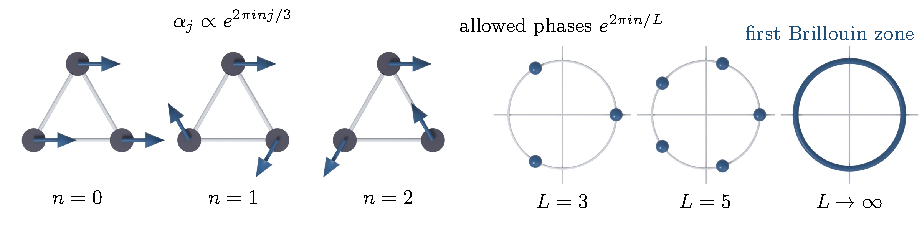
\includegraphics{figures/pdf/s02f01_ringmodes.pdf}
\end{aqmfigure}


\textbf{Five sites on a ring.} The same argument on a five-site ring with nearest-neighbour hopping,
$H=\sum_{\langle ij\rangle} c_i^\dagger c_j$, gives $\varphi_n=2\pi n/5$, $n=0,\dots,4$, and
eigenstates $|\Psi_n\rangle \propto \sum_{j=0}^4 e^{i\varphi_n j}\,c_j^\dagger|0\rangle$. This already
answers a quantitative question without diagonalizing anything: what is the weight of site 1,
in the sense of the overlap $\big|\langle\Omega|c_1\Psi_{\rm GS}^\dagger|\Omega\rangle\big|^2$, in
the lowest-energy eigenstate built from the vacuum $|\Omega\rangle$? Since every $|\Psi_n\rangle$ is
a uniform-modulus superposition over all five sites, this overlap equals $1/5$ for every $n$, lowest
energy or not, purely from the symmetry and with no reference to the specific hopping amplitudes at
all. The same argument survives unchanged even if nearest-neighbour hopping is replaced by
arbitrary long-range hopping (a six-site ring with extra long-range couplings makes the same point):
as long as the ring's rotational symmetry is intact, the symmetry eigenvalues, the eigenstates, and
expectation values like this one are all fixed by symmetry alone, however complicated the
Hamiltonian gets.

It is worth a brief aside that such few-site models are not purely academic. Scanning tunnelling
microscopy can position individual atoms with essentially arbitrary precision, and few-site
tight-binding rings like these have actually been built and measured this way. The famous
stop-motion film built entirely from STM-manipulated atoms, sometimes called ``the smallest film
ever made,'' in which every single dot on screen is an individual atom, is a playful reminder of just
how precisely such models can now be realized in the lab.

\textbf{The infinite chain.} Now let the ring grow without bound, into an infinite one-dimensional chain
with nearest-neighbour hopping. The relevant symmetry is translation by one site, $T: c_n \to
c_{n+1}$, and $[H,T]=0$ for any Hamiltonian built only from hoppings that depend on the distance
between sites, not on absolute position. By Section 2.3, $H$ and $T$ share an eigenbasis, and the
eigenvalue of $T$ on that shared eigenbasis is, by (2.2), a pure phase $e^{i\varphi}$. This
$\varphi$ is the \textbf{Bloch phase}, and the statement that $H$ and $T$ share an eigenbasis, when
applied to a system with translational symmetry, \emph{is} Bloch's theorem: if two operators commute,
there is a common basis for both of them. The mapping between this phase and the corresponding
energy of the Hamiltonian is exactly what we mean by the \textbf{dispersion relation} of a periodic
system.

\section{Bloch's theorem and the first band structure}

Let us make this fully explicit for the one-dimensional tight-binding chain,

\begin{equation}H = -t\sum_n \left(c_n^\dagger c_{n+1} + \text{h.c.}\right).\end{equation}

We take $t>0$ throughout, matching the sign convention of (1.6) in the previous session.

Because $[H,T]=0$, we look for eigenstates built as a translationally-covariant superposition over
all sites,

\begin{equation}|\Psi_\varphi\rangle = \sum_n e^{in\varphi}\, c_n^\dagger|0\rangle.\end{equation}

It is cleanest to invert this relation and define new operators labelled by $\varphi$ instead of by
site,

\begin{equation}\Psi_\varphi^\dagger = \sum_n e^{in\varphi}\, c_n^\dagger, \qquad
c_n^\dagger = \sum_\varphi e^{-in\varphi}\, \Psi_\varphi^\dagger,\end{equation}

an ordinary Fourier transform between real space and the space of Bloch phases. Substituting (2.7)
into (2.5),

\begin{equation*}\sum_n c_n^\dagger c_{n+1} = \sum_{n,\varphi,\varphi'} e^{-in\varphi}\,e^{i\varphi'(n+1)}\,
\Psi_\varphi^\dagger \Psi_{\varphi'} = \sum_{\varphi,\varphi'} e^{i\varphi'}\,\delta_{\varphi\varphi'}\,
\Psi_\varphi^\dagger\Psi_{\varphi'} = \sum_\varphi e^{i\varphi}\, \Psi_\varphi^\dagger\Psi_\varphi,\end{equation*}

where the sum over $n$ produced the orthogonality relation $\sum_n e^{in(\varphi'-\varphi)} =
\delta_{\varphi\varphi'}$. The Hermitian conjugate term contributes the complex conjugate phase, so

\begin{equation}H = -t\sum_\varphi \left(e^{i\varphi}+e^{-i\varphi}\right)\Psi_\varphi^\dagger\Psi_\varphi
= \sum_\varphi \epsilon_\varphi\, \Psi_\varphi^\dagger\Psi_\varphi, \qquad
\boxed{\epsilon_\varphi = -2t\cos\varphi}.\end{equation}

This is our first band structure, obtained without ever writing down, let alone diagonalizing, an
infinite matrix. All we needed was the observation that the eigenstates must carry a definite phase
under translation, and then a single Fourier transform did the rest.

A few features of this dispersion are worth drawing out explicitly, since they recur throughout the
course. Near the band bottom ($\varphi=0$), $\epsilon_\varphi \approx -2t + t\varphi^2$, an
upward-opening parabola; near the band top ($\varphi=\pi$), writing $\varphi=\pi+\delta$,
$\epsilon_\varphi\approx 2t-t\delta^2$, a downward-opening parabola. The two curvatures have
\emph{opposite} sign, which (once effective mass is defined properly in Section 2.9) means low-energy
quasiparticles near the bottom of the band behave like ordinary, positive-mass electrons, while
those near the top behave like negative-mass holes. Near the middle of the band, at $\varphi=\pi/2$
where $\epsilon_\varphi$ crosses zero, the dispersion looks closer to linear than quadratic, a first
hint of the Dirac-like physics we meet properly in Section 2.11. All of this is collected in
figure~\ref{fig:s02:cosband}, which also shows the density of states the band produces.

% Session 2 -- the 1D band, annotated.
% Placement: sec. "Bloch's theorem and the first band structure", after eq. (2.8).
% Rendered by figures/blender/s02f02_cosband.py, labels in figures/overlays/s02f02_cosband.tex.
\begin{aqmfigure}{fig:s02:cosband}{The one-dimensional band $\epsilon_\varphi=-2t\cos\varphi$ of
(2.8), drawn for $t=1$, with the grey tubes showing its local forms. Near the band bottom the
dispersion is an upward parabola, and quasiparticles behave as ordinary electrons with positive
mass. Near the top the curvature has the opposite sign and they behave as holes. Near midband it is
locally linear, which is a first sign of the Dirac physics of Section 2.11. The slope is the group
velocity (2.17) and the curvature is the inverse effective mass (2.18), and both are read from this
one curve. On the right is the resulting density of states (2.16), cut at the top of the drawing,
which diverges at both band edges, at the same points where the group velocity vanishes.}
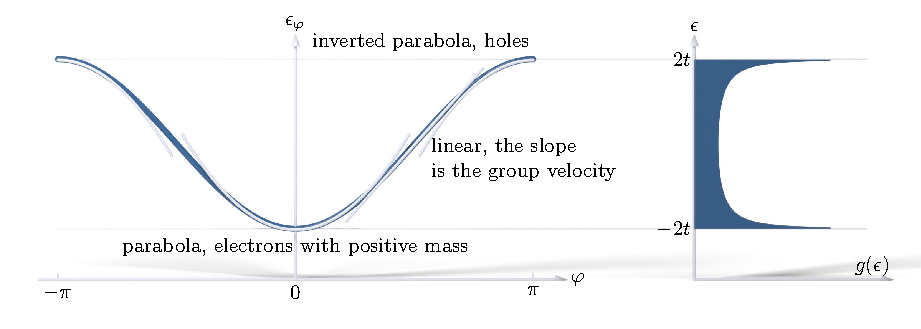
\includegraphics{figures/pdf/s02f02_cosband.pdf}
\end{aqmfigure}


\begin{notebookbox}{\texttt{session2.ipynb}, ``One dimensional chain'' (Core)}
Build exactly the chain of (2.5), diagonalize it numerically, and check that the numerical
spectrum traces out $\epsilon_\varphi=-2t\cos\varphi$ from (2.8) as you scan $\varphi$ across the
Brillouin zone.
\end{notebookbox}

A natural in-class extension checks that the same machinery handles more than nearest-neighbour
hopping. Add a second-neighbour hopping term $-\eta\sum_n(c_n^\dagger c_{n+2}+\text{h.c.})$ to (2.5).
This term has exactly the same translational symmetry as before, so the eigenstates (2.6) are
completely unchanged; only the eigenvalues need recomputing. Repeating the Fourier substitution for
the new term (which pairs $c_n^\dagger$ with $c_{n+2}$, contributing a phase $e^{\pm2i\varphi}$
instead of $e^{\pm i\varphi}$) gives

\begin{equation}\epsilon_\varphi = -2t\cos\varphi - 2\eta\cos(2\varphi).\end{equation}

\begin{notebookbox}{\texttt{session2.ipynb}, ``One dimensional chain, with longer range hopping'' (Core)}
Add the second-neighbour hopping $\eta$ to the chain from the previous callout, and check that the
numerically computed band matches (2.9). It is worth also checking the density of states here
(Section 2.9), since $\eta$ can create a second local extremum in $\epsilon_\varphi$ and, with it,
an extra Van Hove-type feature in the spectrum.
\end{notebookbox}

Also worth flagging by name: \texttt{pyqula}, a Python package that computes band structures like this one
in 1D, 2D, 3D, and beyond, is the computational tool used throughout the course. It appears here only
by name; the slides work through an explicit installation walkthrough (\texttt{pip install pyqula}) and
example scripts for a 1D chain and a 1D two-site-per-cell ``ladder,'' with the resulting band plots
shown on screen. That specific installation walkthrough and its code screenshots are slides-only
material, not narrated in the transcript and not reproduced here; the notebook is where you actually
run the equivalent code yourself.

\section{What the phase means: quasi-momentum}

Let us stop and ask what the phase $\varphi$ in (2.2) physically means, not just formally. Go back to
the continuum Schrödinger equation and ask how translating a wavefunction by the lattice constant
$a$, $\psi(x+a)$, relates to $\psi(x)$. Taylor expanding,

\begin{equation*}\psi(x+a) = \psi(x) + a\,\partial_x\psi(x) + \frac{a^2}{2}\partial_x^2\psi(x) + \cdots
= e^{a\partial_x}\psi(x) = e^{\frac{i}{\hbar}ap}\,\psi(x),\end{equation*}

where $p=-i\hbar\partial_x$ is the momentum operator. If $\psi$ is an eigenstate of the translation
operator with eigenvalue $e^{i\varphi}$, comparing the two expressions identifies

\begin{equation}\varphi = \frac{a\,p}{\hbar} = k\,a,\end{equation}

the symmetry eigenvalue is literally the crystal momentum $k=p/\hbar$ times the lattice constant.
This is why $\varphi$ is called the \emph{quasi-momentum}: it is directly tied to the momentum operator
of the original Schrödinger equation, just measured in units where the lattice constant is
absorbed, and it ranges over $\varphi\in(-\pi,\pi]$, the first Brillouin zone.

This identification also tells us where the orthogonal single-orbital basis we have implicitly been
using comes from. A real material's atomic orbitals, $s$, $p$, $d$, and so on, are not orthogonal
between neighbouring sites; before writing a clean tight-binding Hamiltonian we first pass to an
orthogonalized local basis, one orbital per site, obtained systematically via \textbf{Löwdin
orthogonalization} (a construction the contact session works through properly, and that we simply
assume here; the slides also label this basis ``Wannier states''). In this basis, symmetry alone
already tells us the eigenstates take the form $e^{in\varphi}c_n^\dagger|0\rangle$, exactly the
ansatz (2.6), whether we imagine a finite ring of $7$ sites, $11$ sites, or the infinite chain we
actually want to describe a solid: we can build the same intuition by working through progressively
larger finite rings before taking the $L\to\infty$ limit.

\section{Multi-orbital band structures}

Real unit cells almost never contain a single orbital: graphene has two (one per sublattice),
transition-metal compounds routinely have several $d$-orbitals per site, and so on. Let $\alpha$
label the orbital within a unit cell and $n$ label the unit cell itself. The most general bilinear
Hamiltonian built from these operators, keeping couplings only within a cell and to the
nearest-neighbouring cell (longer-range couplings work by exactly the same trick, just with more
terms), is

\begin{equation}H = \sum_{n,\alpha,\beta} t_{\alpha\beta}\, c_{n,\alpha}^\dagger c_{n,\beta}
+ \sum_{n,\alpha,\beta} \gamma_{\alpha\beta}\, c_{n,\alpha}^\dagger c_{n+1,\beta} + \text{h.c.},
\end{equation}

with $t_{\alpha\beta}$ the intracell hoppings and $\gamma_{\alpha\beta}$ the intercell hoppings.

The symmetry that diagonalizes (2.11) is a slightly richer version of pure translation: it shifts
the unit-cell index $n\to n+1$ \emph{and} performs a unitary rotation among the orbitals within each
cell. The corresponding eigenstates are

\begin{equation*}\Psi_{\varphi,\alpha}^\dagger \sim \sum_{n,\beta} e^{in\varphi}\,U_{\alpha\beta}\,c_{n,\beta}^\dagger,\end{equation*}

for some unitary $U$. Substituting this ansatz into (2.11) and repeating the Fourier argument of
Section 2.5 orbital-by-orbital shows that the required $U$ is exactly the one that diagonalizes the
\textbf{Bloch Hamiltonian}

\begin{equation}H(\varphi) = t + \gamma\, e^{i\varphi} + \gamma^\dagger e^{-i\varphi},\end{equation}

a matrix whose size equals the number of orbitals per unit cell. Each entry is indexed by the pair of
orbitals $(\alpha,\beta)$ it couples: the intracell hoppings $t_{\alpha\beta}$ enter that entry
directly, with no phase, while the intercell hoppings $\gamma_{\alpha\beta}$ enter dressed with the
phase $e^{\pm i\varphi}$ the symmetry eigenvalue provides. This is the general recipe to use again
and again: count orbitals per cell to get the matrix size, place each hopping in the entry its
orbital pair indexes, multiply the intercell ones by $e^{\pm i\varphi}$, and diagonalize. Note that
an intracell hopping between \emph{different} orbitals lands off the diagonal, exactly as the worked
example below shows.

A concrete worked example fixes the idea and will matter again soon. Take a two-orbital ($A,B$)
chain, with strong intracell coupling of magnitude $1$ between $A$ and $B$, and a weaker intercell
coupling $\eta$ linking $B$ in one cell to $A$ in the next. The Bloch Hamiltonian (2.12) is purely
off-diagonal,

\begin{equation}H(\varphi) = \begin{pmatrix} 0 & 1+\eta\,e^{-i\varphi} \\ 1+\eta\,e^{i\varphi} & 0 \end{pmatrix},
\qquad \epsilon_\pm(\varphi) = \pm\left|1+\eta\,e^{-i\varphi}\right|.\end{equation}

This particular alternating-hopping chain is worth remembering by name: it is exactly the
Su-Schrieffer-Heeger-type Hamiltonian that reappears, with a topological twist, in the topology
lecture right after this one. Figure~\ref{fig:s02:recipe} shows the recipe applied to it, matching
each bond of the lattice to the matrix entry it produces, and what happens to the two bands as
$\eta$ is tuned through $1$.

% Session 2 -- from lattice to Bloch Hamiltonian: the recipe.
% Placement: sec. "Multi-orbital band structures", between eqs. (2.12) and (2.13).
%
% NOTE: the intracell hopping t_AB sits OFF the diagonal here -- that is the whole
% point of the annotation, and the reason the adjacent prose was corrected.
%
% The \foreach loop variable is \et, NOT \eta: naming it \eta silently substitutes
% into every "$\eta$" in the panel titles and prints the numeric value instead.
\begin{aqmfigure}{fig:s02:recipe}{Reading a Bloch Hamiltonian off a lattice. The number of orbitals
per unit cell sets the matrix size; an intracell hopping enters the entry its orbital pair indexes
with no phase, an intercell hopping enters the corresponding entry multiplied by $e^{\pm i\varphi}$.
Note that the intracell $A$--$B$ hopping lands \emph{off} the diagonal. For the alternating-hopping
chain (2.13) this gives the two bands $\epsilon_\pm=\pm|1+\eta e^{-i\varphi}|$: gapped for
$\eta\neq1$, and gap-closing exactly at $\eta=1$ -- the Su-Schrieffer-Heeger chain the topology
session picks up.}

\begin{tikzpicture}[x=1cm, y=1cm]

\def\dx{1.55}   % intracell A-B separation
\def\cw{2.65}   % unit-cell period

% ======================= left: the two-orbital chain ========================
\begin{scope}[shift={(0,0)}]
  \node[aqmpanel, anchor=south west] at (-0.75,1.55) {real space};

  % three unit cells
  \foreach \n/\lab in {0/{$n-1$}, 1/{$n$}, 2/{$n+1$}} {
    \begin{scope}[shift={(\n*\cw,0)}]
      \draw[aqmcell] (-0.46,-0.52) rectangle ({\dx+0.55},0.52);
      \node[aqmlabmuted, anchor=north] at ({\dx/2},-1.15) {\lab};
      % strong intracell bond A-B
      \draw[aqmbondstrong, draw=aqmaccent] (0,0) -- (\dx,0);
      \node[aqmsite, minimum size=7pt] at (0,0) {};
      \node[aqmsitealt, minimum size=7pt] at (\dx,0) {};
      \node[aqmlabsmall, anchor=south] at (0,0.12) {$A$};
      \node[aqmlabsmall, anchor=south] at (\dx,0.12) {$B$};
    \end{scope}
  }
  % weak intercell bonds B(n) - A(n+1)
  \foreach \n in {0,1} {
    \draw[aqmbondweak, draw=aqmbroken] ({\n*\cw+\dx},0) -- ({(\n+1)*\cw},0);
  }
  \draw[aqmbondweak, draw=aqmbroken] (-0.68,0) -- (0,0);
  \draw[aqmbondweak, draw=aqmbroken] ({2*\cw+\dx},0) -- ({2*\cw+\dx+0.68},0);

  \node[aqmlabsmall, anchor=south, text=aqmaccent] at ({\cw+\dx/2},0.66)
    {intracell $t_{AB}=1$};
  \node[aqmlabsmall, anchor=north, text=aqmbroken] at ({\cw+\dx+(\cw-\dx)/2},-0.60)
    {intercell $\gamma=\eta$};
\end{scope}

% ======================= right: the Bloch matrix ============================
\begin{scope}[shift={(8.95,0)}]
  \node[aqmpanel, anchor=south] at (1.45,1.55) {Bloch Hamiltonian $H(\varphi)$};

  \node[aqmbox, text width=3.9cm, minimum height=1.5cm] (mat) at (1.45,0)
    {$\displaystyle
      \begin{pmatrix}
        0 & \textcolor{aqmaccent}{1}+\textcolor{aqmbroken}{\eta e^{-i\varphi}}\\[2pt]
        \textcolor{aqmaccent}{1}+\textcolor{aqmbroken}{\eta e^{i\varphi}} & 0
      \end{pmatrix}$};

  \node[aqmlabsmall, anchor=north, align=center, text width=5.0cm] at (1.45,-0.95)
    {\textcolor{aqmaccent}{intracell: no phase}\quad
     \textcolor{aqmbroken}{intercell: $\times\,e^{\pm i\varphi}$}\\[1pt]
     \textcolor{aqmmuted}{matrix size $=$ orbitals per cell $=2$}};
\end{scope}

\draw[aqmarrow] (7.45,0) -- (8.55,0);

% ======================= bottom: the three band panels ======================
\begin{scope}[shift={(0,-6.55)}]
\foreach \px/\et/\ttl/\note in {0/0.45/{$\eta<1$: gapped}/{},
                                4.75/1.0/{$\eta=1$: gap closes}/{gap closes at $\varphi=\pm\pi$},
                                9.50/1.8/{$\eta>1$: gapped again}/{}} {
  \begin{scope}[shift={(\px,0)}]
    \begin{axis}[
      aqmplot,
      width=5.3cm, height=4.3cm,
      title={\ttl},
      xlabel={$\varphi$}, ylabel={$\epsilon_\pm$},
      ylabel style={at={(ticklabel* cs:1.0)}, anchor=south east},
      xmin=-3.9, xmax=3.9, ymin=-3.3, ymax=3.3,
      xtick={-3.14159,0,3.14159}, xticklabels={$-\pi$,$0$,$\pi$},
      ytick=\empty,
      axis lines=middle,
    ]
    % eps_pm = +- |1 + eta e^{-i phi}| = +- sqrt(1 + eta^2 + 2 eta cos phi)
    \addplot[aqmcurve, domain=-3.14159:3.14159, samples=220]
      {sqrt(1 + \et*\et + 2*\et*cos(deg(x)))};
    \addplot[aqmcurve, domain=-3.14159:3.14159, samples=220]
      {-sqrt(1 + \et*\et + 2*\et*cos(deg(x)))};
    % per-panel note, positioned in axis coordinates so it lands correctly
    \node[aqmlabsmall, anchor=north, text=aqmbroken] at (axis cs:0,-2.42) {\note};
    \end{axis}
  \end{scope}
}
\end{scope}

\end{tikzpicture}

\end{aqmfigure}


\begin{notebookbox}{\texttt{session2.ipynb}, ``One dimensional chain, band folding'' (Challenge), and ``One dimensional ladder, band folding'' (Challenge)}
The ``band folding'' section builds exactly this picture from the other direction: take a
single-orbital chain and re-describe it using a larger unit cell (equivalently, more than one
site per cell), and watch a single band from (2.8) fold into multiple bands, as (2.12) predicts.
The ladder section then works through a genuine two-orbital-per-cell model along the lines of
(2.13); check that the numerical bands match $\epsilon_\pm(\varphi)$ there.
\end{notebookbox}

\section{Higher-dimensional band structures}

A two-dimensional lattice has two independent, mutually commuting translations, $T_x$ and $T_y$, so
Bloch eigenstates carry two independent phases, $\varphi_x$ and $\varphi_y$, one per direction, tied
to the crystal momentum along the two lattice vectors by the same Taylor-expansion argument as
(2.10), applied once per direction. The space of allowed $(\varphi_x,\varphi_y)$ pairs is the
\textbf{Brillouin zone}. Because $\varphi=0$ and $\varphi=2\pi$ label the same translation eigenvalue in
both directions, the Brillouin zone is not an open square but a periodic one: identifying the left
and right edges, and the top and bottom edges, turns it into a torus (a circle, in the
one-dimensional case of Section 2.5). This compactness of the Brillouin zone will matter a great deal
once topological invariants enter the next session.

Applying the Fourier trick of Section 2.5 once per spatial direction gives, for a single-orbital
square lattice with nearest-neighbour hopping $t$,

\begin{equation}\epsilon(\varphi_x,\varphi_y) = 2t\left(\cos\varphi_x + \cos\varphi_y\right),\end{equation}

and, applying the identical argument a third time, for a single-orbital cubic lattice,

\begin{equation}\epsilon(\varphi_x,\varphi_y,\varphi_z) = 2t\left(\cos\varphi_x+\cos\varphi_y+\cos\varphi_z\right).
\end{equation}

The same trick extends systematically to four, five, or more dimensions; nothing in the argument
actually depends on being in three-dimensional space. Equations (2.14) and (2.15) are
slides-and-transcript material with no notebook counterpart in \texttt{session2.ipynb}: the notebook's own
two-dimensional worked example goes straight to the honeycomb lattice of Section 2.11 rather than the
plain square lattice, and there is no three-dimensional cubic-lattice section at all. If you want to
check (2.14) or (2.15) numerically, the same construction used for the honeycomb-lattice callout
below extends directly, just with a single-orbital, square (or cubic) Bravais lattice instead.

It is worth being explicit, before moving on, about a point that has been implicit throughout:
everything above applies far beyond electrons. The same Bloch-Hamiltonian trick diagonalizes phonon
bands, magnon bands, and Bogoliubov-de Gennes quasiparticle bands in a superconductor, and it applies
equally well to artificial, engineered lattices, such as cold atoms trapped in optical lattices, that
have nothing to do with real crystals at all. We will focus on electronic bands for concreteness, but
this generality is exactly why the same machinery reappears for magnons, and for Bogoliubov
quasiparticles, later in the course. The physics that comes out of single-particle band theory this
way is itself extremely rich: Dirac fermions with zero effective mass, Weyl semimetals (Dirac points
generalized to higher dimensions), quantum spin Hall insulators, Chern insulators, crystalline
topological phases, and topological superconductors, all of it building on nothing more than the
Bloch Hamiltonian $H(\mathbf{k})$ constructed here.

\section{Properties of an electronic dispersion}

Once we have a dispersion $E(\mathbf{k})$, whether from (2.8), (2.13), (2.14), or something more
elaborate, several derived quantities carry direct physical meaning.

The \textbf{density of states},

\begin{equation}g(\omega) = \int_{\text{BZ}} \frac{d^dk}{(2\pi)^d}\; \delta\!\left(\omega-E(\mathbf{k})\right),
\end{equation}

counts how many states sit at energy $\omega$. It governs how strongly a material responds to
interactions: a large or divergent density of states means even a weak interaction can drive an
instability toward magnetism, a charge density wave, or superconductivity, exactly the three cases
from last session, while a vanishing density of states means interactions struggle to have any effect
at all, however strong.

The \textbf{group velocity},

\begin{equation}v(\mathbf{k}) = \frac{1}{\hbar}\nabla_{\mathbf{k}} E(\mathbf{k}),\end{equation}

is the local slope of the dispersion. Where $v(\mathbf{k})=0$, electrons at that $\mathbf{k}$ are
effectively immobile; where $v(\mathbf{k})$ is large, they propagate through the lattice largely
unaffected by scattering.

The \textbf{effective mass},

\begin{equation}\left(\frac{1}{m^\ast}\right)_{ij} = \frac{1}{\hbar^2}\,
\frac{\partial^2 E(\mathbf{k})}{\partial k_i\,\partial k_j},\end{equation}

is the curvature of the dispersion, and it is the mass actually measured in essentially every
transport or cyclotron-resonance experiment; the bare electron mass is not directly observable
inside a solid. Depending on the band, $m^\ast$ can range from nearly zero to extremely large, or, as
we will see shortly for a Dirac dispersion, formally undefined at the point where the bands touch.

Finally, the \textbf{Fermi surface} is the locus of $\mathbf{k}$-points sharing the energy of the highest
occupied state. Its shape controls which electronic instabilities are favoured, how a material
responds to an external magnetic field, and it is one of the quantities ARPES (Section 2.12) can map
out directly.

\begin{notebookbox}{\texttt{session2.ipynb}, ``Density of states of the honeycomb lattice'' (Core), and ``Fermi surface of the honeycomb lattice'' (Challenge)}
Once the honeycomb dispersion of Section 2.11 is in hand, these two sections let you compute
(2.16) and the Fermi surface directly and see how both change as the Fermi level is tuned through
the Dirac point.
\end{notebookbox}

\section{Three archetypes of dispersion: parabolic, Dirac, and flat}

Real dispersions are complicated functions of $\mathbf{k}$, but almost every band structure in this
course is locally built out of three limiting archetypes.

\begin{enumerate}
\item \textbf{Parabolic bands}, $E\propto k^2$, the free-electron-like case, describe most semiconductors and
   conventional metals. They arise essentially by Taylor expansion near any extremum of a band: we
   already saw this explicitly near $\varphi=0$ and $\varphi=\pi$ in (2.8), with opposite-sign
   effective masses at the two extrema.
\item \textbf{Dirac (linear) dispersions}, $E\propto|k|$, are realized in graphene and in a range of
   topological materials (quantum spin Hall insulators, Chern insulators, and other
   symmetry-protected topological phases). They carry finite topological invariants (a Berry phase)
   and produce phenomenology that echoes relativistic physics, even though the underlying electrons
   are entirely non-relativistic.
\item \textbf{Flat bands}, $E(\mathbf{k})=\text{const}$, might sound like the least interesting case, but by
   (2.16) a flat band produces a \emph{divergent} density of states, so even weak interactions have an
   enormous effect wherever a flat band sits near the Fermi level. When the flatness arises for a
   nontrivial reason, real-space destructive interference rather than simply setting a hopping to
   zero, it can also carry a finite Chern number, central to the quantum Hall effect and to moiré
   materials.
\end{enumerate}

Figure~\ref{fig:s02:archetypes} puts the three side by side with the density of states each one
produces, which is what decides whether interactions can do anything with them.

% Session 2 -- three archetypes of dispersion and the density of states each produces.
% Placement: sec. "Three archetypes of dispersion", alongside the enumerated list.
% Rendered by figures/blender/s02f06_archetypes.py, labels in figures/overlays/s02f06_archetypes.tex.
\begin{aqmfigure}{fig:s02:archetypes}{The three types of dispersion and the densities of states that
they give, all in \emph{two} dimensions. Each band is a surface over the two-dimensional momentum,
with its density of states as a slab next to it on the same energy axis. A parabolic band gives a
constant density of states, which is a step. A Dirac point makes it vanish linearly, so a finite
interaction strength is needed before anything happens. A flat band makes it diverge, drawn here
with a small broadening, so an arbitrarily weak interaction can drive the symmetry-broken states of
Session 1. Almost every band structure in this course is locally one of these three.}
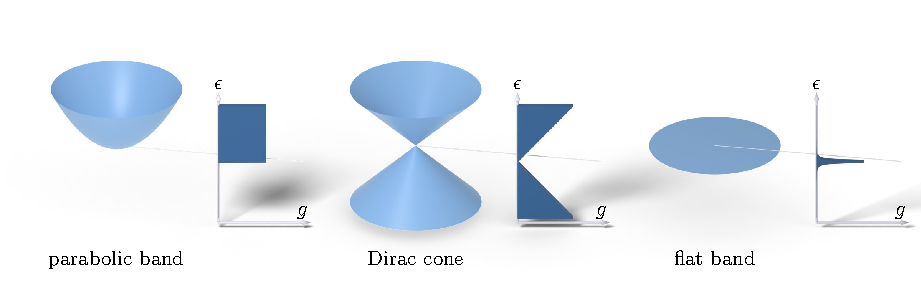
\includegraphics{figures/pdf/s02f06_archetypes.pdf}
\end{aqmfigure}


We derive the Dirac case explicitly next, since it is graphene's defining feature and the direct link
forward to the topology lecture, then look at two lattices that realize flat bands. Both \texttt{pyqula},
introduced by name in Section 2.5, and its GUI companion, a second computational tool shown on the
slides under the name \textbf{Quantum Lattice} (interface-based, no scripting required, and not named
explicitly in speech, which only gestures at ``a user interface we will use at some points''), are the
tools used throughout the course to compute dispersions like these.

\section{The Dirac cone: graphene's honeycomb lattice, and flat-band lattices}

Graphene's honeycomb lattice has two orbitals per unit cell, one on each of two triangular
sublattices, conventionally labelled $A$ and $B$, sitting on an underlying triangular Bravais
lattice. Nearest-neighbour hopping only ever connects $A$ to $B$ (never $A$ to $A$, nor $B$ to $B$),
so by the recipe of Section 2.7 the Bloch Hamiltonian (2.12) is purely off-diagonal,

\begin{equation}H(\mathbf{k}) = \begin{pmatrix} 0 & f(\mathbf{k}) \\ f^\ast(\mathbf{k}) & 0 \end{pmatrix},
\qquad f(\mathbf{k}) = t\sum_{j=1}^{3} e^{i\mathbf{k}\cdot\boldsymbol{\delta}_j},\end{equation}

where $\boldsymbol{\delta}_j$, $j=1,2,3$, are the three vectors connecting an $A$ site to its nearest
$B$ neighbours. Diagonalizing (2.19) gives $E_\pm(\mathbf{k})=\pm|f(\mathbf{k})|$. The function
$f(\mathbf{k})$ vanishes at two inequivalent points of the Brillouin zone, conventionally called $K$
and $K'$, since the three phases in the sum cancel exactly there, and this is why both bands touch at
exactly zero energy at $K$ and $K'$. That cancellation is worth seeing rather than taking on trust:
figure~\ref{fig:s02:dirac} shows the three phase factors at $\mathbf{K}$ as three unit vectors
$120^\circ$ apart, which close a triangle and therefore sum to zero.

% Session 2 -- graphene: three bond vectors, one cancellation, two cones.
% Placement: sec. "The Dirac cone", between eqs. (2.19) and (2.20).
% Rendered by figures/blender/s02f04_dirac.py, labels in figures/overlays/s02f04_dirac.tex.
\begin{aqmfigure}{fig:s02:dirac}{The Dirac cones of graphene. \textbf{(a)} The honeycomb lattice,
with two sublattices $A$, $B$ per unit cell, drawn as dark and grey discs, and the three
nearest-neighbor vectors $\boldsymbol\delta_{1,2,3}$ from an $A$ site. \textbf{(b)} The reason why
the bands touch. At $\mathbf k=\mathbf K$ the three phase factors $e^{i\mathbf
K\cdot\boldsymbol\delta_j}$ are three unit vectors at $120^\circ$ from each other in the complex
plane. When we place them one after the other they close a triangle, so $f(\mathbf K)=0$ in (2.19)
and both bands meet at zero energy. At a generic $\mathbf k$ they do not close, the ghost ball marks
where the sum ends, and the bands are split. \textbf{(c)} The two inequivalent points $K$ and $K'$
of the Brillouin zone with zero energy, at two corners of the hexagonal tile, around which the
dispersion is the linear cone $E_\pm=\pm\hbar v_F|\mathbf q|$ of (2.21).}
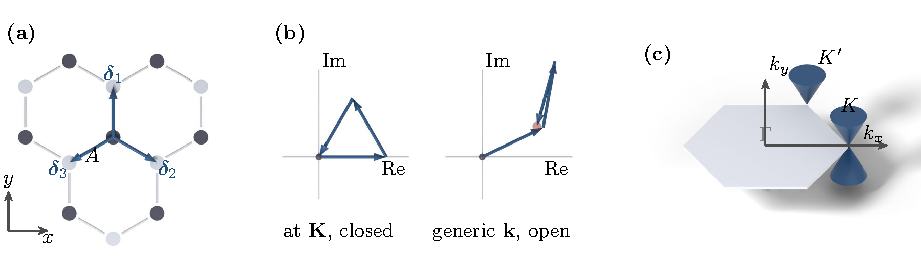
\includegraphics{figures/pdf/s02f04_dirac.pdf}
\end{aqmfigure}


Expanding $f(\mathbf{k})$ to linear order around $K$, writing $\mathbf{k}=\mathbf{K}+\mathbf{q}$ for
small $\mathbf{q}$, the off-diagonal entry becomes a linear function of $\mathbf{q}$ (one linear term
for its real part, one for its imaginary part), and (2.19) reduces to the standard two-dimensional
\textbf{Dirac Hamiltonian},

\begin{equation}H(\mathbf{q}) \approx \hbar v_F\left(q_x\sigma_x + q_y\sigma_y\right), \qquad
v_F = \frac{3ta}{2\hbar},\end{equation}

with $\sigma_x,\sigma_y$ the Pauli matrices acting on the $A/B$ sublattice space and $a$ the
nearest-neighbour bond length. Diagonalizing (2.20) gives

\begin{equation}E_\pm(\mathbf{q}) = \pm \hbar v_F |\mathbf{q}|,\end{equation}

a strictly linear, cone-shaped dispersion around $K$, and by an identical calculation around $K'$:
the \textbf{Dirac cone}. Notice the effective mass from (2.18) is formally zero everywhere on the cone
except exactly at its tip, where it is ill-defined altogether, the ``massless-looking electron''
phenomenology graphene is famous for. This is the low-energy physics of every honeycomb-lattice
material, graphene above all, and there is a great deal more structure hiding at $K$ and $K'$ (a
Berry phase, and with it a topological classification) that we leave for the topology lecture right
after this one.

\begin{notebookbox}{\texttt{session2.ipynb}, ``Infinite two-dimensional graphene'' (Core)}
Build the two-dimensional honeycomb Bloch Hamiltonian (2.19) directly and diagonalize it across
the Brillouin zone. Zoom in on $K$ and $K'$ and check numerically that the dispersion there really
is linear, i.e. that it matches (2.21) once you are close enough to the Dirac point.
\end{notebookbox}

Two standard lattices realize genuinely flat bands from real-space geometry alone, rather than from
any fine-tuning of hopping parameters to zero. The \textbf{Lieb lattice} is built from a square lattice
with one site out of every four removed in a regular pattern; its dispersion has two parabolic bands,
much like the ordinary square lattice (2.14), plus one exactly flat band sitting at zero energy. The
\textbf{kagome lattice} is built instead from a triangular lattice with one site out of every four
removed; it has a dispersion closer to the honeycomb lattice's, hosting Dirac-cone-like linear
crossings, plus, in addition, a flat band at the edge of the spectrum: with the sign convention of
(2.5) it sits at the top, at $\epsilon=2t$, and it would sit at the bottom for the opposite sign of
$t$. In both cases the flat band
arises from destructive interference between hopping paths in real space, a purely geometric effect
rather than an interaction effect (the strong-correlation physics only enters once electrons are
actually placed into these already-flat bands). Figure~\ref{fig:s02:flatbands} shows both lattices,
both dispersions, and the localized state whose hopping paths cancel.

% Session 2 -- flat bands from destructive interference: Lieb and kagome.
% Placement: sec. "The Dirac cone ... and flat-band lattices", at the flat-band passage.
%
% The notes state twice that this content cannot stand without a figure
% ("seeing the actual flat-band dispersion requires the figure itself").
%
% BAND DATA: not hand-derived. Both dispersions were obtained by exact
% diagonalization of the nearest-neighbour Bloch Hamiltonian H = -t sum(c^dag c)
% with t=1, sampled along the high-symmetry path shown, and pasted in as
% coordinates. Lieb: flat band exactly at eps=0, with all three bands touching
% at M. Kagome: flat band at eps=+2t (the TOP of the spectrum for this sign of
% t; it moves to the bottom if the sign of t is flipped), with the two
% dispersive bands meeting in a Dirac-like crossing at K, at eps=-t.
\begin{aqmfigure}{fig:s02:flatbands}{Flat bands that come only from geometry. \textbf{(a)} The Lieb
lattice, which is a square lattice with one site in four removed, and \textbf{(b)} its bands. There
are two dispersive bands and a band that is exactly flat at $\epsilon=0$, and all three touch at $M$.
\textbf{(c)} The kagome lattice, made of triangles that share corners, and \textbf{(d)} its bands,
with a Dirac-like crossing at $K$ and a flat band at $\epsilon=2t$. \textbf{(e)} The reason why the
flat band exists. An eigenstate can be confined to a single kagome hexagon, with amplitudes of
alternating sign around it. Every path by which it could hop onto a site outside arrives twice with
opposite sign, so the two contributions cancel. Nothing is fine-tuned to zero, since the flatness is
a property of the geometry of the lattice, and by (2.16) it makes the density of states diverge.}

\begin{tikzpicture}[x=1cm, y=1cm]

% ============================ (a) Lieb lattice =============================
\begin{scope}[shift={(0,0)}]
  \foreach \i in {0,1,2} {
    \foreach \j in {0,1,2} {
      \draw[aqmbond, draw=aqmmuted, line width=0.5pt]
        (0.7*\i,0.7*\j) -- (0.7*\i+0.7,0.7*\j);
      \draw[aqmbond, draw=aqmmuted, line width=0.5pt]
        (0.7*\i,0.7*\j) -- (0.7*\i,0.7*\j+0.7);
    }
  }
  % corner sites (kept) and edge-centre sites (kept); the plaquette centre is removed
  \foreach \i in {0,1,2,3} { \foreach \j in {0,1,2,3} {
      \node[aqmsite, minimum size=4.6pt] at (0.7*\i,0.7*\j) {}; } }
  \foreach \i in {0,1,2} { \foreach \j in {0,1,2,3} {
      \node[aqmsitealt, minimum size=4pt] at (0.7*\i+0.35,0.7*\j) {}; } }
  \foreach \i in {0,1,2,3} { \foreach \j in {0,1,2} {
      \node[aqmsitealt, minimum size=4pt] at (0.7*\i,0.7*\j+0.35) {}; } }
  \node[aqmpanel, anchor=north] at (1.05,-0.32) {(a) Lieb};
  \node[aqmlabsmall, anchor=north, text=aqmmuted] at (1.05,-0.72) {3 sites per cell};
\end{scope}

% ============================ (b) Lieb bands ===============================
\begin{scope}[shift={(3.35,-0.30)}]
\begin{axis}[
  aqmplot, width=4.9cm, height=3.9cm,
  ylabel={$\epsilon$}, xlabel={},
  ylabel style={at={(ticklabel* cs:1.0)}, anchor=south east, yshift=2pt},
  title={(b) Lieb bands},
  xmin=0, xmax=10.7261, ymin=-3.35, ymax=3.35,
  xtick={0,3.1416,6.2832,10.7261},
  xticklabels={$\Gamma$,$X$,$M$,$\Gamma$},
  ytick={-2.828,0,2.828}, yticklabels={$-2\sqrt{2}t$,$0$,$2\sqrt{2}t$},
  axis lines=left, xmajorgrids, grid style={aqmmuted, line width=0.3pt, dotted},
]
% --- Lieb bands, computed by exact diagonalization of the
% --- nearest-neighbour model H = -t sum(c^dag c), t=1.
% xmax=10.7261 ticks=[(0.0, 'G'), (3.142, 'X'), (6.283, 'M'), (10.726, 'G')]
\addplot[aqmcurve] coordinates {(0.000,-2.828) (0.136,-2.825) (0.271,-2.815) (0.407,-2.799) (0.542,-2.777) (0.678,-2.749) (0.814,-2.715) (0.949,-2.677) (1.085,-2.633) (1.220,-2.586) (1.356,-2.535) (1.492,-2.482) (1.627,-2.426) (1.763,-2.370) (1.899,-2.314) (2.034,-2.260) (2.170,-2.207) (2.305,-2.159) (2.441,-2.115) (2.577,-2.076) (2.712,-2.045) (2.848,-2.021) (2.983,-2.006) (3.119,-2.000) (3.232,-1.998) (3.368,-1.987) (3.503,-1.967) (3.639,-1.939) (3.774,-1.901) (3.910,-1.854) (4.046,-1.799) (4.181,-1.736) (4.317,-1.665) (4.452,-1.586) (4.588,-1.499) (4.724,-1.406) (4.859,-1.307) (4.995,-1.201) (5.131,-1.090) (5.266,-0.974) (5.402,-0.853) (5.537,-0.729) (5.673,-0.601) (5.809,-0.470) (5.944,-0.337) (6.080,-0.203) (6.215,-0.068) (6.347,-0.064) (6.539,-0.255) (6.731,-0.446) (6.922,-0.634) (7.114,-0.819) (7.306,-1.001) (7.498,-1.178) (7.690,-1.349) (7.881,-1.514) (8.073,-1.673) (8.265,-1.824) (8.457,-1.966) (8.648,-2.099) (8.840,-2.223) (9.032,-2.336) (9.224,-2.439) (9.416,-2.530) (9.607,-2.610) (9.799,-2.678) (9.991,-2.733) (10.183,-2.776) (10.374,-2.807) (10.566,-2.824)};
\addplot[aqmcurvebroken, line width=1.6pt] coordinates {(0.000,0.000) (0.136,0.000) (0.271,0.000) (0.407,0.000) (0.542,0.000) (0.678,0.000) (0.814,0.000) (0.949,0.000) (1.085,0.000) (1.220,0.000) (1.356,0.000) (1.492,0.000) (1.627,0.000) (1.763,0.000) (1.899,0.000) (2.034,0.000) (2.170,0.000) (2.305,0.000) (2.441,0.000) (2.577,0.000) (2.712,0.000) (2.848,0.000) (2.983,0.000) (3.119,0.000) (3.232,0.000) (3.368,0.000) (3.503,0.000) (3.639,0.000) (3.774,0.000) (3.910,0.000) (4.046,0.000) (4.181,0.000) (4.317,0.000) (4.452,0.000) (4.588,0.000) (4.724,0.000) (4.859,0.000) (4.995,0.000) (5.131,0.000) (5.266,0.000) (5.402,0.000) (5.537,0.000) (5.673,0.000) (5.809,0.000) (5.944,0.000) (6.080,0.000) (6.215,0.000) (6.347,0.000) (6.539,0.000) (6.731,0.000) (6.922,0.000) (7.114,0.000) (7.306,0.000) (7.498,0.000) (7.690,0.000) (7.881,0.000) (8.073,0.000) (8.265,0.000) (8.457,0.000) (8.648,0.000) (8.840,0.000) (9.032,0.000) (9.224,0.000) (9.416,0.000) (9.607,0.000) (9.799,0.000) (9.991,0.000) (10.183,0.000) (10.374,0.000) (10.566,0.000)};
\addplot[aqmcurve] coordinates {(0.000,2.828) (0.136,2.825) (0.271,2.815) (0.407,2.799) (0.542,2.777) (0.678,2.749) (0.814,2.715) (0.949,2.677) (1.085,2.633) (1.220,2.586) (1.356,2.535) (1.492,2.482) (1.627,2.426) (1.763,2.370) (1.899,2.314) (2.034,2.260) (2.170,2.207) (2.305,2.159) (2.441,2.115) (2.577,2.076) (2.712,2.045) (2.848,2.021) (2.983,2.006) (3.119,2.000) (3.232,1.998) (3.368,1.987) (3.503,1.967) (3.639,1.939) (3.774,1.901) (3.910,1.854) (4.046,1.799) (4.181,1.736) (4.317,1.665) (4.452,1.586) (4.588,1.499) (4.724,1.406) (4.859,1.307) (4.995,1.201) (5.131,1.090) (5.266,0.974) (5.402,0.853) (5.537,0.729) (5.673,0.601) (5.809,0.470) (5.944,0.337) (6.080,0.203) (6.215,0.068) (6.347,0.064) (6.539,0.255) (6.731,0.446) (6.922,0.634) (7.114,0.819) (7.306,1.001) (7.498,1.178) (7.690,1.349) (7.881,1.514) (8.073,1.673) (8.265,1.824) (8.457,1.966) (8.648,2.099) (8.840,2.223) (9.032,2.336) (9.224,2.439) (9.416,2.530) (9.607,2.610) (9.799,2.678) (9.991,2.733) (10.183,2.776) (10.374,2.807) (10.566,2.824)};
\node[aqmlabsmall, anchor=west, text=aqmbroken] at (axis cs:0.4,0.42) {flat band};
\end{axis}
\end{scope}

% ============================ (c) kagome lattice ===========================
\begin{scope}[shift={(8.55,0)}]
  % corner-sharing triangles: draw up- and down-triangles on a triangular lattice
  \foreach \i in {0,1,2} {
    \foreach \j in {0,1} {
      \pgfmathsetmacro\ox{0.72*\i + 0.36*\j}
      \pgfmathsetmacro\oy{0.624*\j}
      \draw[aqmbond, draw=aqmmuted, line width=0.5pt]
        (\ox,\oy) -- ++(0.72,0) -- ++(-0.36,0.624) -- cycle;
      \draw[aqmbond, draw=aqmmuted, line width=0.5pt]
        (\ox+0.36,\oy+0.624) -- ++(0.72,0) -- ++(-0.36,-0.624) -- cycle;
    }
  }
  \foreach \i in {0,1,2,3} {
    \foreach \j in {0,1,2} {
      \pgfmathsetmacro\ox{0.72*\i + 0.36*\j}
      \pgfmathsetmacro\oy{0.624*\j}
      \node[aqmsite, minimum size=4.2pt] at (\ox,\oy) {};
      \node[aqmsite, minimum size=4.2pt] at (\ox+0.36,\oy) {};
    }
  }
  \node[aqmpanel, anchor=north] at (1.05,-0.32) {(c) kagome};
  \node[aqmlabsmall, anchor=north, text=aqmmuted] at (1.05,-0.72) {3 sites per cell};
\end{scope}

% ============================ (d) kagome bands =============================
\begin{scope}[shift={(11.90,-0.30)}]
\begin{axis}[
  aqmplot, width=4.9cm, height=3.9cm,
  ylabel={$\epsilon$}, xlabel={},
  ylabel style={at={(ticklabel* cs:1.0)}, anchor=south east, yshift=2pt},
  title={(d) kagome bands},
  xmin=0, xmax=9.4029, ymin=-4.5, ymax=2.9,
  xtick={0,3.1416,5.5654,9.4029},
  xticklabels={$\Gamma$,$M$,$K$,$\Gamma$},
  ytick={-4,-1,2}, yticklabels={$-4t$,$-t$,$2t$},
  axis lines=left, xmajorgrids, grid style={aqmmuted, line width=0.3pt, dotted},
]
% --- Kagome bands, computed by exact diagonalization of the
% --- nearest-neighbour model H = -t sum(c^dag c), t=1.
% xmax=9.4029 ticks=[(0.0, 'G'), (3.142, 'M'), (5.565, 'K'), (9.403, 'G')]
\addplot[aqmcurve] coordinates {(0.000,-4.000) (0.136,-3.995) (0.271,-3.982) (0.407,-3.959) (0.542,-3.927) (0.678,-3.886) (0.814,-3.837) (0.949,-3.779) (1.085,-3.713) (1.220,-3.639) (1.356,-3.558) (1.492,-3.469) (1.627,-3.374) (1.763,-3.272) (1.899,-3.165) (2.034,-3.052) (2.170,-2.934) (2.305,-2.812) (2.441,-2.686) (2.577,-2.558) (2.712,-2.426) (2.848,-2.293) (2.983,-2.158) (3.119,-2.023) (3.211,-2.005) (3.316,-2.012) (3.421,-2.018) (3.525,-2.024) (3.630,-2.030) (3.734,-2.035) (3.839,-2.039) (3.944,-2.042) (4.048,-2.044) (4.153,-2.045) (4.258,-2.044) (4.362,-2.043) (4.467,-2.040) (4.571,-2.035) (4.676,-2.030) (4.781,-2.023) (4.885,-2.014) (4.990,-2.004) (5.095,-1.993) (5.199,-1.981) (5.304,-1.968) (5.408,-1.953) (5.513,-1.938) (5.621,-1.921) (5.786,-1.922) (5.952,-1.963) (6.118,-2.040) (6.283,-2.145) (6.449,-2.268) (6.615,-2.404) (6.780,-2.547) (6.946,-2.693) (7.111,-2.838) (7.277,-2.981) (7.443,-3.119) (7.608,-3.250) (7.774,-3.374) (7.940,-3.489) (8.105,-3.594) (8.271,-3.688) (8.437,-3.771) (8.602,-3.842) (8.768,-3.900) (8.934,-3.945) (9.099,-3.977) (9.265,-3.995)};
\addplot[aqmcurve] coordinates {(0.000,2.000) (0.136,1.995) (0.271,1.982) (0.407,1.959) (0.542,1.927) (0.678,1.886) (0.814,1.837) (0.949,1.779) (1.085,1.713) (1.220,1.639) (1.356,1.558) (1.492,1.469) (1.627,1.374) (1.763,1.272) (1.899,1.165) (2.034,1.052) (2.170,0.934) (2.305,0.812) (2.441,0.686) (2.577,0.558) (2.712,0.426) (2.848,0.293) (2.983,0.158) (3.119,0.023) (3.211,0.005) (3.316,0.012) (3.421,0.018) (3.525,0.024) (3.630,0.030) (3.734,0.035) (3.839,0.039) (3.944,0.042) (4.048,0.044) (4.153,0.045) (4.258,0.044) (4.362,0.043) (4.467,0.040) (4.571,0.035) (4.676,0.030) (4.781,0.023) (4.885,0.014) (4.990,0.004) (5.095,-0.007) (5.199,-0.019) (5.304,-0.032) (5.408,-0.047) (5.513,-0.062) (5.621,-0.079) (5.786,-0.078) (5.952,-0.037) (6.118,0.040) (6.283,0.145) (6.449,0.268) (6.615,0.404) (6.780,0.547) (6.946,0.693) (7.111,0.838) (7.277,0.981) (7.443,1.119) (7.608,1.250) (7.774,1.374) (7.940,1.489) (8.105,1.594) (8.271,1.688) (8.437,1.771) (8.602,1.842) (8.768,1.900) (8.934,1.945) (9.099,1.977) (9.265,1.995)};
\addplot[aqmcurvebroken, line width=1.6pt] coordinates {(0.000,2.000) (0.136,2.000) (0.271,2.000) (0.407,2.000) (0.542,2.000) (0.678,2.000) (0.814,2.000) (0.949,2.000) (1.085,2.000) (1.220,2.000) (1.356,2.000) (1.492,2.000) (1.627,2.000) (1.763,2.000) (1.899,2.000) (2.034,2.000) (2.170,2.000) (2.305,2.000) (2.441,2.000) (2.577,2.000) (2.712,2.000) (2.848,2.000) (2.983,2.000) (3.119,2.000) (3.211,2.000) (3.316,2.000) (3.421,2.000) (3.525,2.000) (3.630,2.000) (3.734,2.000) (3.839,2.000) (3.944,2.000) (4.048,2.000) (4.153,2.000) (4.258,2.000) (4.362,2.000) (4.467,2.000) (4.571,2.000) (4.676,2.000) (4.781,2.000) (4.885,2.000) (4.990,2.000) (5.095,2.000) (5.199,2.000) (5.304,2.000) (5.408,2.000) (5.513,2.000) (5.621,2.000) (5.786,2.000) (5.952,2.000) (6.118,2.000) (6.283,2.000) (6.449,2.000) (6.615,2.000) (6.780,2.000) (6.946,2.000) (7.111,2.000) (7.277,2.000) (7.443,2.000) (7.608,2.000) (7.774,2.000) (7.940,2.000) (8.105,2.000) (8.271,2.000) (8.437,2.000) (8.602,2.000) (8.768,2.000) (8.934,2.000) (9.099,2.000) (9.265,2.000)};
\node[aqmlabsmall, anchor=south east, text=aqmbroken] at (axis cs:8.55,2.12) {flat band};
\node[aqmlabsmall, anchor=west, align=left] at (axis cs:5.75,-1.02)
  {\footnotesize Dirac};
\end{axis}
\end{scope}

% ================= (e) the localized flat-band state =======================
\begin{scope}[shift={(4.55,-4.35)}]
  \node[aqmpanel, anchor=south] at (0.9,1.45) {(e) why the band is flat: destructive interference};

  % a kagome hexagon: six sites at 60-degree steps
  \def\hr{1.02}
  \foreach \k in {0,...,5} { \coordinate (h\k) at ({60*\k}:\hr); }
  \foreach \k in {0,...,5} {
    \pgfmathtruncatemacro\kk{mod(\k+1,6)}
    \draw[aqmbondstrong, draw=black] (h\k) -- (h\kk);
  }
  % alternating amplitudes +1 / -1 around the loop
  \foreach \k in {0,2,4} {
    \node[circle, draw=aqmbroken, fill=aqmfillb, line width=0.9pt,
          minimum size=13pt, inner sep=0pt, font=\footnotesize] at (h\k) {$+$};
  }
  \foreach \k in {1,3,5} {
    \node[circle, draw=aqmaccent, fill=aqmfill, line width=0.9pt,
          minimum size=13pt, inner sep=0pt, font=\footnotesize] at (h\k) {$-$};
  }
  \node[aqmlabsmall, align=center] at (0,0) {amplitude\\[-2pt]$\pm1$};

  % an outside site, reached from two hexagon sites of opposite sign
  \coordinate (out) at ({\hr*1.86},{\hr*0.52});
  \node[aqmsiteopen, minimum size=8pt] at (out) {};
  \draw[aqmbondweak, draw=aqmmuted] (h0) -- (out);
  \draw[aqmbondweak, draw=aqmmuted] (h1) -- (out);
  \node[aqmlabsmall, anchor=north west, align=left, text width=4.6cm] at ({\hr*2.05},{\hr*0.72})
    {the two hopping paths onto this site arrive with amplitudes
     $-t(+1)$ and $-t(-1)$:\\[2pt]
     \textbf{they cancel exactly}\\[2pt]
     \textcolor{aqmmuted}{the state cannot leak out, so its energy does not
     depend on $\mathbf k$ -- a flat band}};
\end{scope}

\end{tikzpicture}

\end{aqmfigure}


This is slides-only material with no notebook counterpart in \texttt{session2.ipynb}: the notebook works
through the honeycomb lattice in depth but has no Lieb-lattice or kagome-lattice section of its own.
The band-structure plots for both lattices are shown directly on the slides; the description above
captures their qualitative structure, but seeing the actual flat-band dispersion requires the figure
itself.

\section{Measuring band structures: ARPES}

A natural question, once all this formalism is in hand, is whether any of it is actually observable.
The energy eigenvalue $E(\mathbf{k})$ is clearly physical, but the quasi-momentum $\mathbf{k}$ itself
started life as a symmetry eigenvalue in Section 2.6; is it something we can measure directly, and can
we measure the \emph{relation} between the two?

The answer is yes, via \textbf{angle-resolved photoemission spectroscopy (ARPES)}. The idea is
conceptually simple: shoot photons of known energy and momentum at a material; each photon can eject
an electron from the material entirely (the photoelectric effect), and momentum and energy
conservation relate the electron's momentum and kinetic energy, both measured directly outside the
material, back to its momentum and energy while still inside. Scanning the emission angle and
kinetic energy of the ejected electrons therefore maps out $E(\mathbf{k})$ directly. This is exactly
how the graphene band structure and Fermi surface are measured in practice, and the measured Dirac
cone matches the tight-binding derivation of Section 2.11 closely. This is slides-only material with
no notebook counterpart: the actual ARPES images of graphene's measured band structure and Fermi
surface are shown on the slides, and there is no way to reproduce a real photoemission experiment in
a tight-binding notebook; the description above captures the physical principle, but seeing the
measured data itself requires the figure.

\section{Closing summary}

\begin{itemize}
\item \textbf{Symmetry as a simplification tool.} When the ground state shares the Hamiltonian's symmetry, we
  can use a commuting symmetry operator, $[H,S]=0$ in (2.3), to find $H$'s eigenbasis by finding
  $S$'s eigenbasis instead, a strategy worked through explicitly for rings of three and five sites in
  Section 2.4.
\item \textbf{Bloch's theorem} is exactly this idea applied to translational symmetry on an infinite lattice:
  eigenstates carry a definite phase $\varphi$ (the quasi-momentum, (2.10)) under translation, turning
  one infinite-dimensional diagonalization into a continuous family of finite ones, the \textbf{Bloch
  Hamiltonian} $H(\varphi)$.
\item We derived the one-dimensional chain's band structure explicitly, $\epsilon_\varphi=-2t\cos\varphi$
  in (2.8), and generalized the same machinery to second-neighbour hopping (2.9), multiple orbitals
  per unit cell via the matrix Bloch Hamiltonian $H(\varphi)=t+\gamma e^{i\varphi}+\text{h.c.}$ in
  (2.12)-(2.13), and higher spatial dimensions, (2.14) and (2.15).
\item A dispersion $E(\mathbf{k})$ determines a material's measurable properties directly: density of
  states (2.16), group velocity (2.17), effective mass (2.18), and Fermi surface, and every real
  dispersion is locally built from three archetypes: parabolic, Dirac, and flat.
\item The \textbf{Dirac cone} of graphene's honeycomb lattice, $H(\mathbf{q})\approx\hbar v_F(q_x\sigma_x+
  q_y\sigma_y)$ with $E_\pm=\pm\hbar v_F|\mathbf{q}|$ in (2.20)-(2.21), is this session's single most
  important worked example, derived directly from the vanishing of the off-diagonal Bloch Hamiltonian
  (2.19) at the $K,K'$ points; the Lieb and kagome lattices realize flat bands by the same kind of
  real-space interference, with no fine-tuning required.
\item All of this band-structure machinery generalizes directly to phonons, magnons, and
  Bogoliubov-de Gennes quasiparticles, not just electrons, and is checked against real materials
  experimentally via ARPES.
\end{itemize}

If there is one thing to take away: periodic-system spectra are computed via band-structure theory by
choosing the shared eigenbasis of the symmetry operator and the Hamiltonian, and the resulting
$E(\mathbf{k})$ dispersion relation determines a great deal about a material's electronic properties
on its own, before interactions ever re-enter the picture. The Dirac cone derived in Section 2.11 is
not just graphene trivia: it is exactly the object the next session picks up and asks what happens
when you gap it open, which is where topological band structure, Chern numbers, and the SSH model
(already glimpsed in the two-orbital chain of (2.13)) all enter the course in earnest. Flat bands,
too, are not the end of the story: the kagome and Lieb constructions here are the direct predecessor
of the Landau-level flat bands the quantum Hall session builds several sessions from now.
